\chapter{Technical Issues}\label{chapter:technicalissues}
This chapter covers some of the problems encountered when turning the model from Chapter \ref{chapter:model} into code. This is not an exhaustive list but focuses on the more interesting problems and solutions. A look at the final software design is yet to come in Chapter \ref{chapter:softwaredesign} so this chapter does not make too many explicit references to the actual classes and methods used and instead tries to focus more on the algorithms and frameworks used.

  \section{ABM frameworks}
    \subsection{What is an ABM framework?}
    The first challenge was to create a software environment to run the simulation. Agent-based modelling (ABM) frameworks handle the creation of such an environment. In particular for this simulation, they break down time  into discrete ticks, during which methods scheduled on objects will run. There also provide a way to display the movement of objects about a 2D space.
    
    \subsection{Why use an ABM framework?}
    Gilbert and Bankes (\cite{Gilbert2002}) discuss the advantages and
    disadvantages of using pre-existing libraries and frameworks for ABM rather
    than ``rolling your own.'' Using pre-existing libraries frees a
    programmer up from re-implementing common
    algorithms. However, they also require a programmer to understand the
    language they are written in and to work with the built-in
    assumptions used by the original writers. Gilbert and Bankes state
    that agent-based modeling tools that match their ideal specifications
    do not yet exist but that there is a trend towards better
    tools becoming available. Fortunately a few years later Allen (\cite{Allan2009}) and Berryman (\cite{Berryman2008}) survey ABM frameworks and suggest that Repast Simphony (the latest version of Repast), MASON and NetLogo are useful tools.
    
    \subsection{ABM frameworks considered}
    \subsubsection{Repast Simphony}
    \begin{itemize}
      \item Open source so it is easy to inspect what the framework is doing behind the scenes.
      \item Java-based so can use any Java library in the agents.
      \item Well documented and has an active mailing list (\cite{Repast}).
      \item There are useful examples to be found on the web such as Nick Malleson's RepastCity (\cite{Malleson}).
      \item Integrates nicely with Eclipse so easy to install and quick to get started.
    \end{itemize}    
        
    \subsubsection{MASON}
    MASON is similar to Repast Simphony (in fact it was designed as an alternative to Repast(\cite{Allan2009})). It is also Java-based and open source. It is designed to be faster than Repast and ``excels'' in its support for learning algorithms (\cite{Berryman2008}).
      
    \subsubsection{NetLogo}
    The main of advantage of NetLogo is its simplicity to use for people without programming experience and to this end NetLogo uses of a proprietary language to program the agents aimed at beginner programmers. However, this language is restrictive compared to a heavily-used language like Java.
    
    \subsection{ABM framework chosen}
    With only a few months to complete this project but a good understanding of Java, using a pre-built framework would require less work than starting from the bottom and building a framework dedicated to the project. The simplicity of NetLogo ruled it out. In the end Repast was chosen. Berryman finds little to separate MASON and Repast Simphony. The integration with Eclipse made getting started with Repast Simphony easy. The improved random number support according to \cite{} would be useful for running experiments, where control over random number streams was essential to ensure reproducibility. Although Repast Simphony does have support for learning algorithms, the improved support in MASON might be missed but their use was a nice-to-have at the planning stage for this project rather than an essential. Also as the simulation would not have to handle a large number of agents (1000 boats would fill the river entirely), the optimizations in MASON would not be necessary. Finally the personal recommendation and one-to-tutorial with EngD student Ed Manley (\cite{Manley2012}) at UCL working on traffic simulations proved sufficient enough reason to confirm the choice of using Repast Simphony over MASON.
  
  \section{Action execution}
    Each tick the cox chooses and executes an action and then the boat moves forward based on the state the cox's action have left the boat. The execution of actions by the cox provided a few problems. Firstly, it was  necessary to decide what period of time each of these ticks covers. Then it was necessary to ensure that if an action was misused (for instance executed in a situation where it did not make sense) then it would not break the system. Finally boats needed to react to a cox's actions rather than allowing the cox too much direct control over the boat in order to help maintain the indirectness of a cox's control over a boat in the implementation.
    
    \subsection{Time discretization and scale}
    An obvious choice was to make each tick stand for one second. This meant it was possible to store distances as metres and speeds as metres per second in a natural way. Fortunately this choice of tick length also worked well with the visualization as Repast offered a way to put delays between the ticks so that a simulation can either be run very quickly through to it being possible to watch it in an equivalent to real time. This tick length also meant a boat would move a relatively short distance each tick so movement appears smooth and there is less danger of getting into unusual situations of boats jumping long distances.
    
    \subsection{Ensuring misuse of action does not break system}
      Ideally a cox would not choose to execute an action in a situation where it did not make sense. Unfortunately this is not possible to ensure without artificially limiting a cox's choices. Instead if an action is executed in a non-conforming situation (for example, trying to change lanes when already in the process of changing lanes) the action will revert to a default action. The Let Boat Run action fits nicely as this default action, since it results in the boat continuing forward unchanged. In a way this is equivalent to a cox deciding to carry out an action and then realising it is not possible.

    \subsection{Separating cox's actions and boat's ``reaction"}
    Separate scheduled methods on cox and boat objects means that the cox's method can concentrate on the cox's actions. The boat's method will then ensure, whatever the cox decides, that the boat will continue to move forward. In turn, this means that the methods for moving a boat can be shielded from the cox so reduce the risk of a cox's actions influencing the movement of a boat too directly. 
    
    The one exception to this was the Spin action. For visualization purposes it was necessary to have the boat rotate 180\textdegree while moving in a straight-line across the river, which was very different to the usual boat movement straight forward in the direction the boat was facing. Therefore it was easier for this one off case to have the Spin action call movement methods directly on the boat object. This actually fits nicely with reality where during spinning the cox does tend to control the boat more directly by calling each stroke individually.

      Repast has a mechanism for setting the priority of scheduled methods. This means that cox's decision making method can be executed before the boat's movement method and so ensure that the boat's movement will be affected by the cox's decision.

      \subsubsection{Actions taking multiple time ticks}
      Some actions by the cox are considered to take multiple time ticks. Spinning is the example. By making each action a class and execution of an action occurring by instantiating an instance of the relevant class and calling the \texttt{execute()} method which returns a boolean to determine whether the action was completed, it was possible to keep a reference to any unfinished actions. These unfinished actions can then be continued at the time tick without the danger of the cox choosing another action which would not make sense. For example, until spinning is complete, it makes no sense to execute any other action.
  
    \section{Visualization}
      It was important for this project to have a visualization. Most importantly the visualization allows anyone to observe the effects of particular control policies. It is easy to spot where bottlenecks in traffic flow might be occurring and occasionally the cause (perhaps by not allowing boats to overtake, a single slow boat holds up everyone? perhaps by allowing boats to crash into each other, a large pile up occurs at the lock where boats take a long time to spin). A visualization was also a useful tool for debugging the simulation and ensuring that the boats where behaving as expected. Fortunately Repast provides a API to visualize the changes to objects each tick - in this case to show where the boats have moved to on the river each tick.

      The visualization has two main elements. The static river and the moving boats. Drawing the river provided a large challenge covered in its own section (see Section \ref{techissues:river}). Drawing the boats was not without problems despite how easy Repast makes it to show objects moving around a continuous 2D space. Originally the boats were all red rectangles. This made them very simple to draw. However these rectangles were not particularly intuitive to look at and they presented two problems:
      \begin{enumerate}
        \item \label{techissues:visualization:boat_shape} It was not possible to tell which way boat was pointing.
        \item \label{techissues:visualization:boat_colour} The boats could be hard to tell apart from each other since they were the same colour. 
      \end{enumerate}
      As with the river, problem \ref{techissues:visualization:boat_shape} was solved using Java's Path2D API to draw a more appropriate shape with 8 oars and a pointed bow to point forwards. Problem \ref{techissues:visualization:boat_colour} was solved by giving each boat a randomly selected colour. These can be seen in Figure \ref{techissues:fig:boats}.

      \begin{figure}
      \begin{center}
        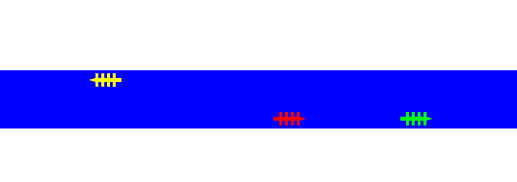
\includegraphics[scale=0.3]{images/boats.png}
        \caption{Multi-coloured boats: notice the shape of the boat with 8 spines to represent the 8 oars. The front of the boat points forward, while the back is flat.}
        \label{techissues:fig:boats}
      \end{center}
      \end{figure}
  
  \section{Building the river}\label{techissues:river}
    The river presented two challenges. Even with the decision to represent it in the model as three graphs to represent the three lanes there was still the challenge of determining the value of the location attribute for each node. Then there was the problem of drawing this river in the visualization.
    
    \subsection{Rastorization vs vectorization}
      Early models of the river had it as an open space in which a
      boat was free to move. Therefore it seemed easier to store the
      river for visualization as a series of squares (effectively
      pixels). This made collision detection with the bank easier
      (only had to check that the whole boat was on the finite number
      of river squares). Unfortunately it was not possible to
      represent this easily in Repast. Repast can draw the grid and
      keep track of which were river squares and which were
      not. However, it could not do this in an efficient manner and
      would recalculate the value of the square at each tick. Also it
      was difficult to draw smooth corners in this manner.
      
      The solution came with the idea to treat the river as 3 lanes that was described in Chapter \ref{chapter:model}. Each lane is then drawn using series of vectors between each node. Since the nodes should be a fixed 20m apart within a lane, it is only necessary to calculate the angle of the vector from one node to the next. The location of a point 5m to each side of the node was stored in order to get a 2D outline of each lane as well as storing the location of the node in the graph in the middle of the lane. These three locations were determined by taking the three points (20, 5), (20, 0) and (20, -5) and rotating them by the angle associated with the next vector and then translating them by the location of the last placed node. 
      
      The outline of the river as a whole was then calculated by using the top boundary of the top lane and the bottom boundary of the bottom lane. The Path2D.Double class in Java made it easy to form and draw this arbitrary shape which Repast was then able to display. 
      
      The next challenge was to work out the number of vectors to use and the heading of each one . The algorithm used to calculate these follows. 
      
      \subsubsection{General algorithm for calculating the heading of each vector}
      First split the river up into straight sections and corners connecting them. 
      
      The vectors that make up all three lanes of a straight section all have the same angle. The number of vectors is the length of the straight section is the length of the straight divided by the length of each vector (so 20m in this case). Google Earth made it easy to determine the length and heading of each straight with it's ruler tool.
      
      Corners are treated as arcs of circles. The following steps give a way to estimate the number and heading of  vectors that makes up a corner.
      
      \begin{enumerate}
        \item Calculate the angle of the sector of a circle whose arc the corner matches. This is the difference of the headings of the straights on either side of the corner
        
        \item Calculate the radius of this sector. This radius will differ between lanes. The radius to the outer lane will the 10m larger than to the middle lane and the radius of the inner lane will be 10m smaller than the radius to the middle lane. 
        
        \item Calculate the length of each of the 3 arcs (one for each lane) with the angle of the sector and the radii of each of the lanes. If the angle is in radians this is angle $\times$ radius.
        
        \item Calculate the number of vectors required to make up each arc. This is length of arc divided by the length of a vector. 
        
        \item The angle of the first vector is the angle straight entering the corner
        
        \item For each of the next vectors increment the angle by (total angle of sector)/(number of segments) each time. Therefore the last segment will have an angle roughly that of the next straight.
      \end{enumerate}
      
       It is worth drawing the output for each corner as the lanes can get slightly out of sync due to rounding errors and so may need an edge added by hand.
      
      \subsubsection{Worked example for the simplified version of Cam used in simulation}
      Google Earth provided the tools for getting the inputs for the algorithm just described.
      
      Figure \ref{techissues:fig:actualcam} highlights an aerial photo of the part of the Cam in which we are interested. The three main corners are labelled. In our simplification of the Cam the segments between the corners are considered as straight.
      
      \begin{figure}
      \begin{center}
        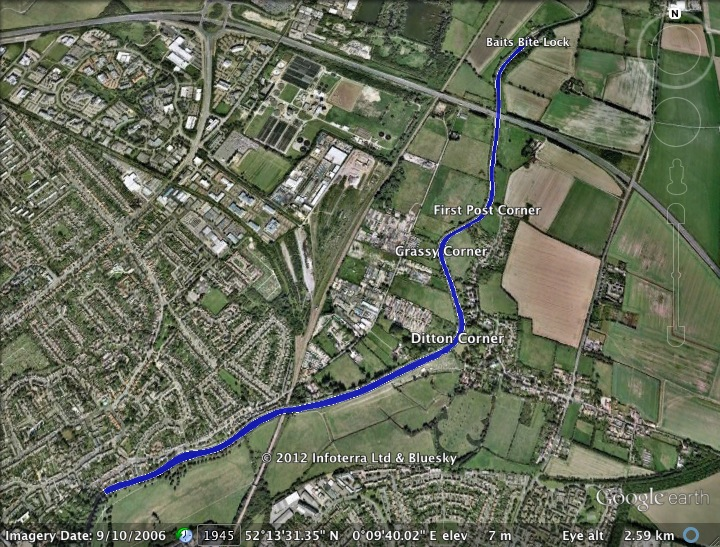
\includegraphics[scale=0.3]{images/GoogleEarthCam.png}
        \caption{The part of the Cam covered by this project marked out on Google Earth. The 3 main corners and Baits Bite Lock have been marked out.}
        \label{techissues:fig:actualcam}
      \end{center}
      \end{figure}
      
      For this worked example, we will follow the algorithm the straight heading into Ditton Corner and that corner itself.
      
      We assumed the three lanes start at (10,10), (10,20), (10,30) in the co-ordinate system for the simulation. Figure \ref{fig:thereach} shows a  screen shot of Google Earth of this first section of river. The ruler tool in Google Earth shows this straight is roughly 1400m long. This corresponds to 70 vectors each 20m long. Although the bearing of this straight is roughly 70\textdegree, for simplicity we treat this first straight as heading due East (so a heading of 0\textdegree from the origin). Everything else in the simulated version of the Cam will be rotated to match.
      
      \begin{figure}
      \begin{center}
        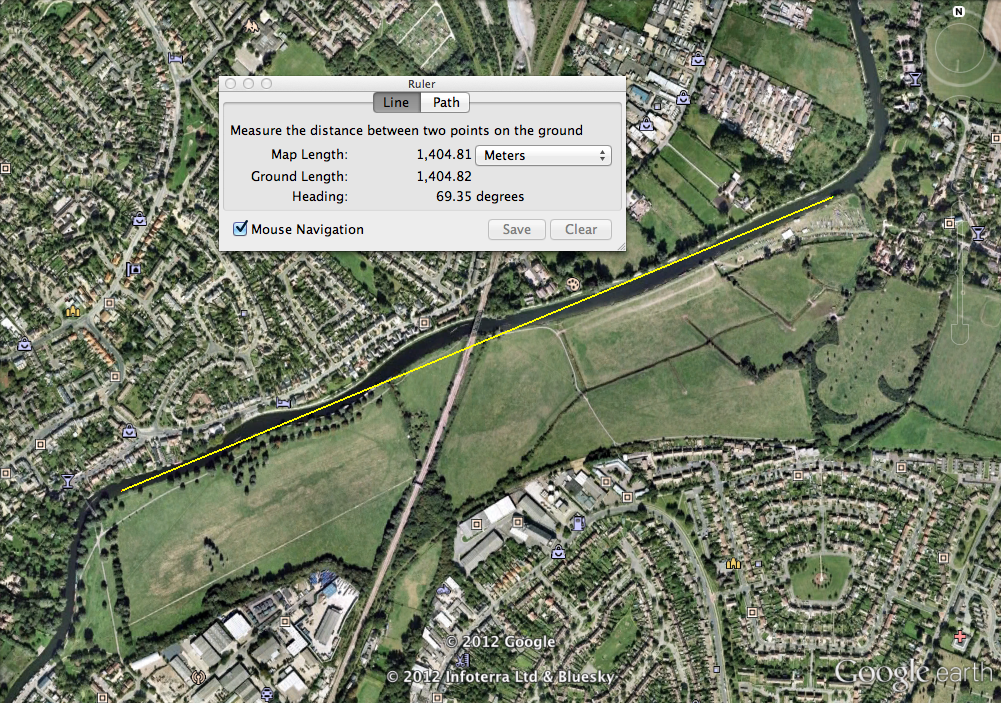
\includegraphics[scale=0.3]{images/TheReach.png}
        \caption{The Reach: roughly 1400m long and straight. By rotating the whole river 20\textdegree \ clockwise can treat it as 70 lots of 20m vectors heading having an angle of 0\textdegree \ from the horizontal (the line apporoximation in Google Earth has a heading of 70\textdegree but this is a bearing so measured clockwise from North unlike standard geometry which measures anti-clockwise from the $x$-axis.)}
        \label{fig:thereach}
      \end{center}
      \end{figure}
      
      Next we look at Grassy Corner. Figure \ref{fig:dittoncorner:angle} shows that the bearing on one side is roughly 250\textdegree\  and on the other roughly 350\textdegree. To simplify the calculations we will treat this corner as 90\textdegree\ (or $\frac{\pi}{2}$ radians).
      
      \begin{figure}
      \begin{center}
        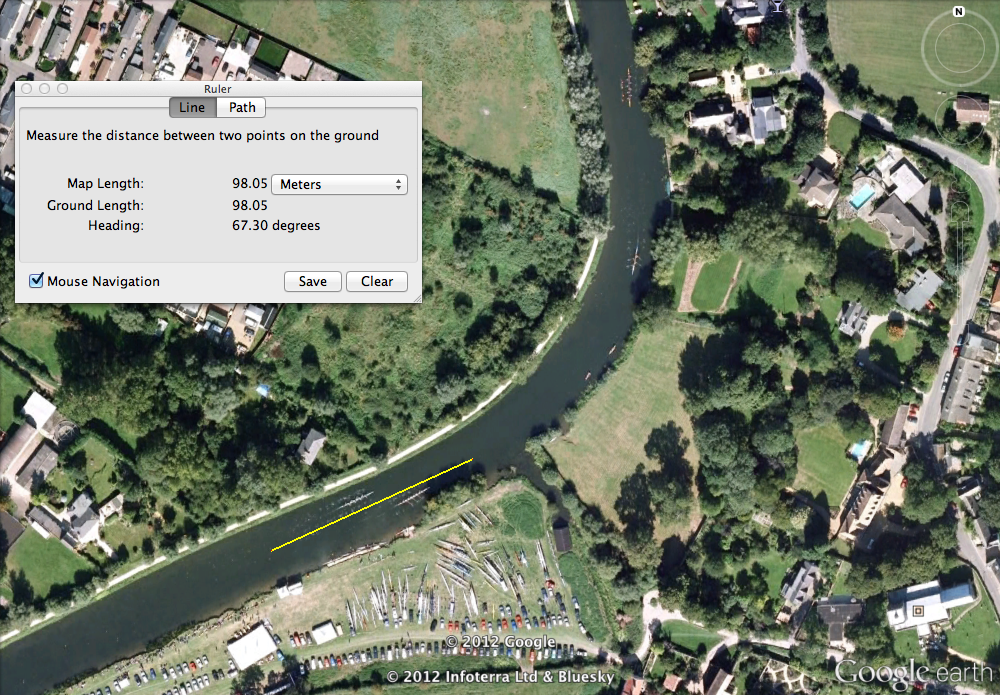
\includegraphics[scale=0.3]{images/DittonCornerHeadingIn.png}
        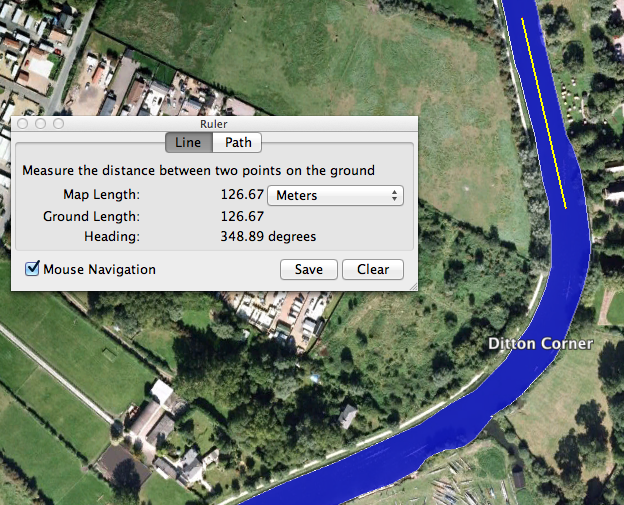
\includegraphics[scale=0.3]{images/DittonCornerHeadingOut.png}
        \caption{Ditton Corner: The heading in is roughly 70\textdegree and the heading out is roughly 170\textdegree so treated this corner as a 90\textdegree sector of a circle (by using a right-angle the calculations were a bit simpler).}
        \label{fig:dittoncorner:angle}
      \end{center}
      \end{figure}
      
      \begin{figure}
      \begin{center}
        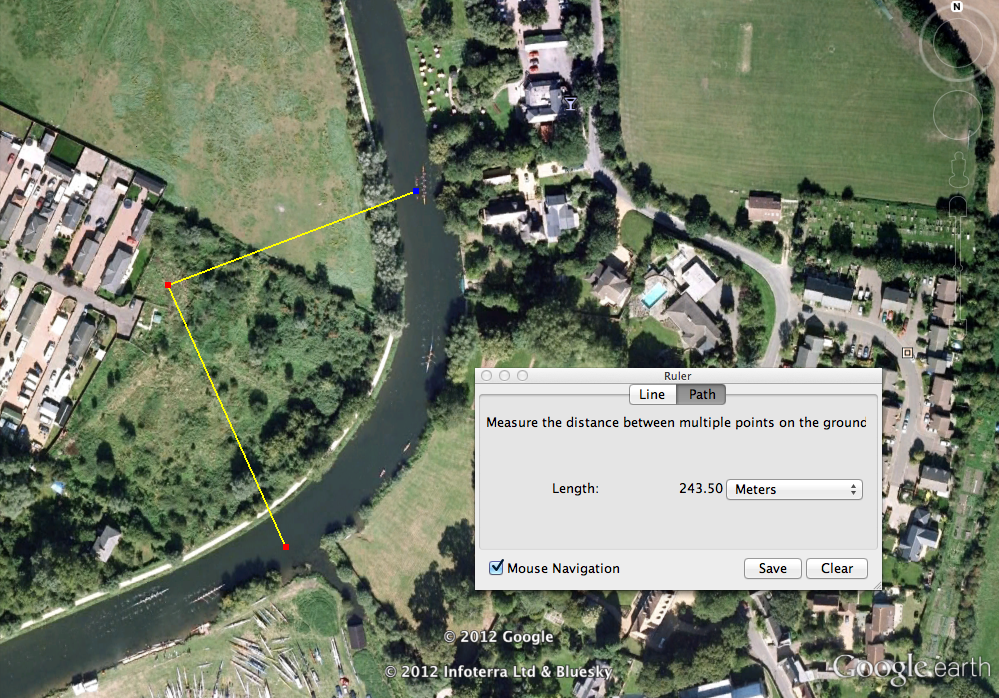
\includegraphics[scale=0.3]{images/DittonCornerRadius.png}
        \caption{Ditton Corner: This shows two approximate radii of the sector that makes up Ditton Corner. Their total length is 202m. Rounded this down, the approximated the radius of Ditton Corner is 100m.}
        \label{fig:dittoncorner:radius}
      \end{center}
      \end{figure}
      
      Figure \ref{fig:dittoncorner:radius} shows a rough outline of two radii that make up the sector. The two radii are approximately 200m long, so a single radius is 100m long. This is for the middle of the river. The radius of the upper lane should be 10m less than this in the 3 lane approximation. And the radius of the lower lane should be 10m more.
      
      Therefore the length of the arcs are roughly $\frac{90\pi}{2}$m, $\frac{100\pi}{2}$m, $\frac{110\pi}{2}$m for the inside, middle and outside lanes respectively. So we need roughly seven, eight and nine 20m-vectors to make up the inside, middle and outside lanes of this corner. Therefore the angle of each vector increments in steps of 0.22, 0.20 and 0.17 radians respectively.
      
      Repeating this procedure for the rest of the area marked out on Google Earth in Figure \ref{techissues:fig:actualcam} and the river is turned into the simplified version displayed in Figure \ref{techissues:fig:simplecam}.
      
      \begin{figure}
      \begin{center}
        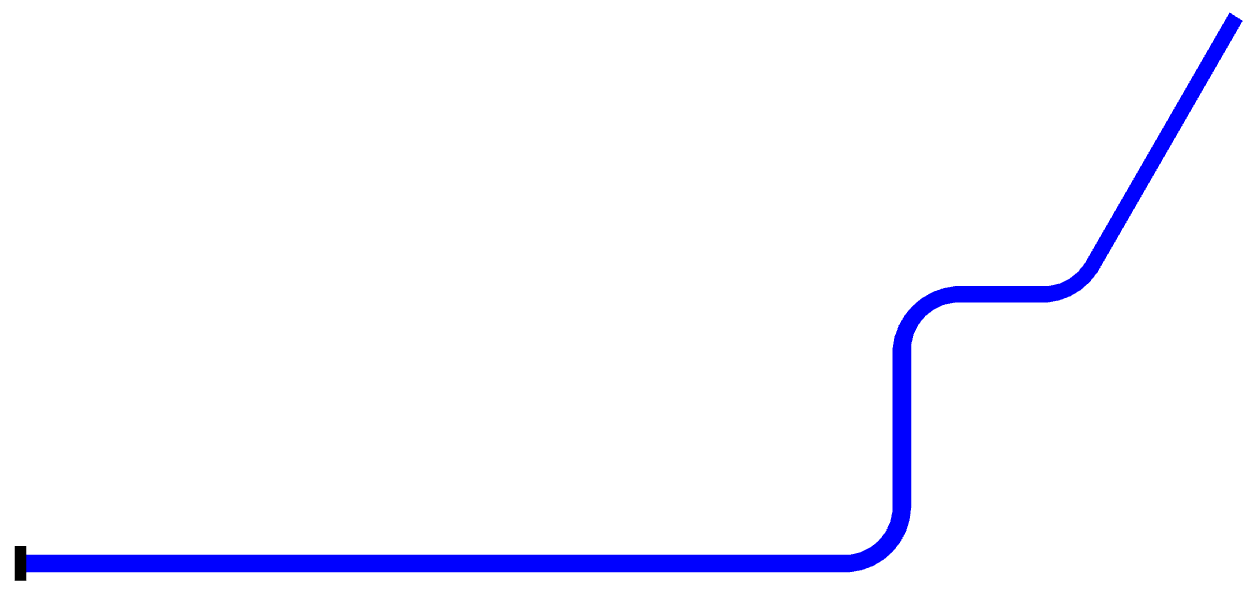
\includegraphics[scale=0.3]{images/SimplifiedCam.png}
        \caption{The simplified version of the Cam as it appears in the visualization. Notice the three corners. The black box represents the boathouse.}
        \label{techissues:fig:simplecam}
      \end{center}
      \end{figure}
      
  \section{Experiment Framework}
  In order to evaluate the control policies it was necessary to run
  experiments and collect data. There are two phases to the
  experiments. First an experiment needs to be setup which includes
  scheduling boats to be launched and their launch
  parameters. Secondly, while the simulation runs, data about the boats needs to be collected such as how many times they crash and how many ticks it takes for each to complete their outing and return to the boathouse. Both these were achieved using a MySQL database despite Repast having both a batch run environment where many simulations can be run with varying parameters and a mechanism to collect data during a simulation run. 
  
  Storing data for setting up and experiment and data collected during an experiment in a database meant it was easy to organise the data and ensure it persisted so the same experiment could be run multiple times and their results compared. As each experiment requires parameters for each boat launched, a database provided an easier way to organise many schedules with lots of launches compared to setting many parameters (each launch has 5 parameters and a schedule has tens of launches and each experiment will try multiple schedules with multiple random keys) in a batch run. 
  
  Repast's data collection only allowed outputting the data to a file. Although Repast offered file formats such as csv, a database offered a much easier way to create a structured, permanent record of experimental data for later analysis.
  
  \subsection{Simulation Run Setup}
  Each run of the simulation in an experiment uses a set of parameters which corresponds to a row in the database with fields for storing the random seed, the control policy the coxes should follow and the schedule to follow. A schedule consists of a set of boat launches to schedule along with the parameters to use. These parameters are the minimum distance the boat should cover in the outing (which for this project was constant at 5000m, roughly equivalent to a run to the lock and back), the speed multiplier (again for this project a constant at 0.5, which meant a boat in gear 10 would travel at 5m/s which roughly matches the 6.3m/s of the world record over 2km), the gear the boat would ideally travel in and the tick the boat should be launched at.
  
  Experiments and launch schedules based on parameters such as number of boats to launch and delay between each launch can be created using simple scripts. The creation of schedules is completely independent to running the simulation. All that matters is the data ends up in the database. This meant it was easy to write the scripts using Ruby. The ease-of-use of the Ruby language and the object relational mapper (ORM) Active Record made it very quick to write these scripts which can quickly create new schedules. This was much simpler than using a Java ORM like Hibernate which requires endless configuration.
  
  When each simulation begins it checks a parameter called Simulation Parameters Id and looks up the row in the database corresponding to this simulation parameters id. It then looks up the scheduled launches associated with this set of simulation parameters and schedules the \texttt{launch()} method to run on the boathouse object with the launch parameters set in the database at the appropriate ticks.
  
    An example set of simulation parameters might be the use the SafetyFocussed control policy, with a random seed of 1132785369 and a schedule that launches 10 boats with a 10 minute interval between each launch. Table \ref{technicalissues:simulation_parameters:schedule} holds an example of the parameters used with each launch.
    
    \begin{table}[h]
    \centering
    \csvreader[tabular=|c|c|c|c|,
        table head=\hline Launch second & Desired Gear For Boat & Distance To Cover & Speed Multiplier\\\hline,
        late after last line=\\\hline]
{csv/ExampleLaunchSchedule.csv}{launch_tick=\tick,desired_gear=\gear,speed_multiplier=\multiplier,distance_to_cover=\distance}
    {\tick & \gear & \distance & \multiplier}
    \caption{An example set of launch parameter for 10 boats launched with a 10 minute interval.}
    \label{technicalissues:simulation_parameters:schedule}
    \end{table}
  
  \subsection{Data Collection}
  While an experiment runs, data collected is stored in the database. A record of the parameters used at each stage (like the random seed and launch tick of each boat) is stored. Therefore if an experiment or schedule is edited there is still an accurate record of what happened. Plus new data is generated such as how far the boat actually moved and the number of crashes that occurred. Repast allows the scheduling of methods to run at the end of a simulation run. One was setup to flush all the data collected to the database. Since this occurs in the simulation, JDBC is used to connect to the database in Java. Although this requires a bit more work writing SQL queries compared to Ruby and ActiveRecord, since the simulation was creating the data the process of adding the data to the database was not as complicated as generating schedules and so it was not a large problem.
  
  Methods were added to the simulation to generate the data.
  \begin{itemize}
    \item Each time a crash occurs the crash counter of the in progress experiment is incremented.
    \item At the end of a boat's scheduled \texttt{run()} method is a call to a method which updates that boat's records with information like how far the boat had now moved in total.
    \item When a boat landed, it's record would be flushed to the database to reduce the amount of data that had to be flushed at the end and to ensure that some data is in the database in case something went wrong later in the simulation.
  \end{itemize}
  
  In this way it is straight-forward to set up new experiments and keep a permanent record of any data collected during the experiment.

